% !TEX spellcheck = en-US
\documentclass{llncs}
%

\usepackage{amssymb}
\usepackage{color}
\usepackage{graphics}
\usepackage{latexsym}
\usepackage{algorithm}
\usepackage{amsfonts}
\usepackage{amsmath}
\usepackage{float}
\usepackage{tabularx}
\usepackage{subcaption}
\usepackage{hyperref}
\usepackage{graphicx}
\usepackage{float}
\usepackage{tikz}
\usepackage{bm}
\usepackage{tikz-qtree}
\usetikzlibrary{patterns}
\usetikzlibrary{positioning}
\usetikzlibrary{arrows,automata,calc,backgrounds,fit,shapes,shapes.gates.logic.US,shapes.gates.logic.IEC,calc,shapes.misc,circuits.logic.US}
\usepackage{centernot}
\usetikzlibrary{shapes.misc}
\usepackage{pifont}
\usepackage{array}
\usepackage{stmaryrd}
\usepackage{tikz}
\usepackage{xcolor}
\usetikzlibrary[arrows]
\usepackage{multirow}
\usepackage{caption}
\usepackage{adjustbox}

\newcommand*\rot[2]{\multicolumn{1}{R{#1}{#2}}}% no optional argument here, please!
\newcommand{\vars}{\textit{Vars}}
\newcommand{\values}{\textit{Val}}
\newcommand{\lb}{\llbracket}
\newcommand{\rb}{\rrbracket}
\newcommand{\mods}[2]{[#2]_{#1}}
\newcommand{\dn}[1]{D\llbracket #1 \rrbracket}
\newcommand{\Rank}[1]{\hspace{3pt} \pmb{\langle} #1 \pmb{\rangle}\hspace{3pt} } % {\triangleright}
\newcommand{\areth}{\lozenge}
\newcommand{\comp}{\blacklozenge}
\newcommand{\States}{\Omega}
\newcommand*{\xMin}{0}%
\newcommand*{\xMax}{7}%
\newcommand*{\yMin}{0}%
\newcommand*{\yMax}{7}%
\colorlet{lightgray}{gray!10}

\newfloat{program}{thp}{lop}
\floatname{program}{Program}

\bibliographystyle{splncs03}

\begin{document}

\title{RankPL: A Qualitative Probabilistic Programming Language}

\author{Tjitze Rienstra}
\institute{University of Luxembourg\\ \email{tjitze@gmail.com}}


\maketitle

\begin{abstract}
In this paper we introduce \emph{RankPL}, a modeling language
	that can be thought of as a qualitative variant of a probabilistic programming language
	with a semantics based on Spohn's ranking theory.
Broadly speaking, RankPL can be used to represent and reason about processes that exhibit 
	uncertainty expressible by distinguishing ``normal'' from ``surprising'' events.
RankPL allows (iterated) revision of rankings over alternative program traces and
	supports various types of reasoning, including abduction and causal inference.
We present syntax and semantics, 
	demonstrate the language with practical examples,
	and discuss an implementation that we made available for download.
\end{abstract}

\section{Introduction}

\emph{Probabilistic programming languages} (PPLs) are regular programming languages extended with statements to 
	(1) draw values at random from a given probability distribution, and 
	(2) condition values of variables due to observation.
Running a probabilistic program yields, instead of a deterministic outcome, a probability distribution over possible outcomes.
PPLs greatly simplify the problem of representing and reasoning with rich probabilistic models 
	and have received increasing attention in recent years, mainly in the context of Bayesian machine learning.
Examples of PPLs include Church~\cite{DBLP:conf/uai/GoodmanMRBT08}, 
	Venture~\cite{DBLP:journals/corr/MansinghkaSP14} and Figaro~\cite{pfeffer2009figaro}.
Early work on PPLs goes back to Kozen~\cite{DBLP:journals/jcss/Kozen81}.
%\emph{Probabilistic programming languages} (PPLs) are general purpose programming languages extended with statements to 
%	(1) draw values at random from a given probability distribution, and 
%	(2) condition values of variables due to observation.
%While regular programs are deterministic and represent single outcomes, 
%	probabilistic programs represent probability distributions over possible outcomes.
%PPLs greatly simplify the problem of representing and reasoning with rich probabilistic models 
%	and have received increasing attention in recent years, mainly in the context of Bayesian machine learning.
%Examples of PPLs include Church~\cite{DBLP:conf/uai/GoodmanMRBT08}, 
%	Venture~\cite{DBLP:journals/corr/MansinghkaSP14} and Figaro~\cite{pfeffer2009figaro}.
%Early work on PPLs goes back to Kozen~\cite{DBLP:journals/jcss/Kozen81}, 

\emph{Ranking theory} is a qualitative abstraction of probability theory in which events receive discrete degrees of surprise called \emph{ranks}~\cite{DBLP:books/daglib/0035277}.
That is, events can be ranked 0 (not surprising), 1 (surprising), 2 (very surprising), and so on, or $\infty$ if impossible.
Ranking theory is computationally simpler than probability theory and does not require precise probabilities to perform meaningful inference. 
Still, it provides analogues to many powerful probabilistic notions, including conditioning and independence.
Ranking theory has been applied in logic-based AI approaches 
		such as belief revision and non-monotonic reasoning~\cite{DBLP:dblp_journals/ai/DarwicheP97,goldszmidt1996qualitative} 
		as well as formal epistemology~\cite{DBLP:books/daglib/0035277}.\looseness=-1
%\emph{Ranking theory} is a qualitative abstraction of probability theory in which events are associated with discrete \emph{ranks}
%	that represent degrees of surprise or inverse degrees of plausibility.
%Thus, an event can be ranked 0 (not surprising), 1 (surprising), 2 (very surprising), and so on; or $\infty$, which designates impossibility.
%Ranking theory is computationally simpler than probability theory and does not require precise probabilities
%	to perform meaningful inference. 
%At the same time, it provides analogues to many powerful notions 
%	known from probability theory, such as conditioning, independence 
%	and Bayesian networks.
%Ranking theory is applied logic-based AI approaches 
%	such as belief revision and non-monotonic reasoning~\cite{DBLP:dblp_journals/ai/DarwicheP97,goldszmidt1996qualitative},
%	as well as mathematical philosophy~\cite{DBLP:books/daglib/0035277}.

In this paper we develop a language called RankPL.
Semantically, the language draws a parallel with probabilistic programming in terms of ranking theory.
We start with a minimal imperative programming language (\textbf{if-then-else}, \textbf{while}, etc.)
	and extend it with statements to
	(1) draw choices at random from a given ranking function and
	(2) perform ranking-theoretic conditioning on values of variables due to observation.
Analogous to probabilistic programs, RankPL programs represent ranking functions over possible outcomes.

Broadly speaking, RankPL can be used to represent and reason about processes
	whose input or behavior exhibits uncertainty expressible % in terms of rankings, or expressible 
	by distinguishing normal (rank $0$) from surprising (rank $> 0$) events.
%This includes ranking networks (i.e., the ranking-based counterpart of Bayesian networks),
%Examples are systems based on ranking networks 
%	(the ranking-based counterpart of Bayesian networks) and ranking-based Markov chains.
%A high degree of modelling flexibility is provided TODO: improve
%	such as those involving a temporal dimension or large state spaces.
Reasoning tasks that are supported include causal inference, abduction and different types of (iterated) belief revision.
The latter are consistent with the AGM postulates for belief revision and DP postulates for iterated belief revision~\cite{DBLP:dblp_journals/ai/DarwicheP97,Gardenfors:1995:BR:216136.216138}.
Just as PPLs provide a high degree of flexibility in reasoning about rich probabilistic models, RankPL does so for ranking-theoretic models.
%These tasks can be implemented without having to write inference-specific code.

The overview of this paper is as follows.
Section~\ref{sec:rankingtheory} deals with basics of ranking theory.
In section~\ref{sec:rpl} we introduce RankPL and present its syntax and semantics.
This is a \emph{denotational} semantics, which defines the meaning of a statement in terms of a ranking transformation function.
In section~\ref{sec:noisy} we discuss two generalized conditioning schemes (L-conditioning and J-conditioning) and show how they can be implemented in RankPL.
All the above will be demonstrated by practical examples of RankPL programs.
In section~\ref{sec:implementation} we discuss our RankPL implementation 
	and conclude in section~\ref{sec:conclusion}.
%These two special constructs are, of course, very similar to those used to define PPLs,
%	except that they work with ranks instead of probabilities.
%Any ranking function over valuations (i.e., assignments of values to variables of the program) can be represented by a ranked program.
%Ranking networks (the ranking-equivalent of Bayesian networks~\cite{goldszmidt1996qualitative,DBLP:books/daglib/0035277}) can be represented by combining 
%	ranked choice with sequences of \textbf{if}-\textbf{then}-\textbf{else} statements.
%The \textbf{while} construct makes it easy to represent still more complex models, 
%	such as those involving a temporal dimension or large state spaces.
%Just as PPLs provide a high degree of flexibility in representing probabilistic models, RankPL does so for ranking-theoretic models.
%All this will be demonstrated in due course.

%\subsection{Belief revision}

%As we mentioned, one area where ranking theory has been applied is belief revision.
%Belief revision is concerned with the question of how to revise a belief set $K$ by 
%	a new sentence $\phi$ (possibly inconsistent with $K$) so as to obtain a new 
%	belief set $K * \phi$ that incorporates $\phi$.
%This problem is usually approached by focusing on postulates that characterize classes of well-behaved revision operators.
%The most-studied set of such postulates are the so called AGM postulates~\cite{Gardenfors:1995:BR:216136.216138}.
%Ranking theory, on the other hand, provides a constructive model for belief revision.
%It has been shown, for example, that ranking-theoretic conditioning satisfies all the essential AGM postulates.
%Moreover, ranking theory provides an elegant solution to the problem of \emph{iterated} belief revision TODO finish.

%What does this mean in the context of RankPL?
%Because the \textbf{observe} statement corresponds to ranking-theoretic conditioning,
%	we have the ability to perform belief revision during the execution of a program.
%Intuitively, if the zero-ranked outcomes of a program represent its \emph{expected} behaviour,
%	then the observe statements allows us to revise this expectation on the basis of new information.
%This is a form of revision that is completely consistent with the AGM postulates.
%
%But there is more.
%TODO: iterated revision
 
%\subsection{Plan of the paper}

%As a formal foundation for RankPL we develop a denotational semantics,
%	which defines the meaning of a RankPL statement as a function that transforms ranking functions over valuations.
%This semantics can be thought of as the ranking-based variation of the denotational semantics for 
%	probabilistic programs due to Kozen~\cite{DBLP:journals/jcss/Kozen81}.
%We then show how iterated revision operators can be represented in RankPL.
%TODO
%
%We also developed an implementation of RankPL.
%It is written in Java an can be used either as an interpreter of the language as we present
%	it in this paper, or in an embedded fashion, where RankPL programs
%		can interact with Java code.
%We describe this implementation in section TODO.
%
%Before we move on, we present a short overview of ranking theory.

\section{Ranking Theory}\label{sec:rankingtheory}

Here we present the necessary basics of ranking theory, all of which is due to Spohn~\cite{DBLP:books/daglib/0035277}.
The definition of a \emph{ranking function} presupposes a finite set $\Omega$ of possibilities
	and a boolean algebra $\mathcal{A}$ over subsets of $\Omega$, which we call \emph{events}.

\begin{definition}
A ranking function is a function $\kappa: \Omega \rightarrow \mathbb{N} \cup \{\infty\}$ that associates every possibiltiy with a \emph{rank}.
$\kappa$ is extended to a function over events by defining $\kappa(\emptyset) = \infty$ and $\kappa(A) = min( \{ \kappa(w) \mid w \in A \} )$ for each $A \in \mathcal{A} \setminus \emptyset$.
A ranking function must satisfy $\kappa(\Omega) = 0$.
\end{definition}

As mentioned in the introduction, ranks can be understood as degrees of surprise or, alternatively, as inverse degrees of plausibility.
The requirement that $\kappa(\Omega) = 0$ is equivalent to the condition that at least one $w \in \Omega$ receives a rank of 0.
We sometimes work with functions $\lambda: \Omega \rightarrow \mathbb{N} \cup \{\infty\}$ that violate this condition.
The \emph{normalization} of $\lambda$ is a ranking function denoted by $|| \lambda ||$ and defined by $|| \lambda ||(w) = \lambda(w) - \lambda(\Omega)$.
Conditional ranks are defined as follows.

\begin{definition}\label{def:conditional}
Given a ranking function $\kappa$, the rank of $A$ conditional on $B$ (denoted $\kappa(A \mid B)$ is defined by
\[
                \kappa(A \mid B) = \left\{ \begin{array}{ll}
                 \kappa(A \cap B) - \kappa(B)& \mbox{if $\kappa(B) \not = \infty$,} \\
                 \infty & \mbox{otherwise.} \\
                   \end{array}
                  \right. \\
\] 
We denote by $\kappa_{B}$ the ranking function defined by $\kappa_{B}(A) = \kappa(A \mid B)$.
\end{definition}

In words, the effect of conditioning on $B$ is that the rank of $B$ is shifted down to zero (keeping the relative ranks of the possibilities in $B$ constant) 
	while the rank of its complement is shifted up to $\infty$.

How do ranks compare to probabilities?
An important difference is that ranks of events do not add up as probabilities do.
That is, if $A$ and $B$ are disjoint, then $\kappa(A \cup B) = min(\kappa(A), \kappa(B))$, while $P(A \cup B) = P(A) + P(B)$.
This is, however, consistent with the interpretation of ranks as degrees of surprise (i.e., $A \cup B$ is no less surprising than $A$ or $B$).
Furthermore, ranks provide deductively closed beliefs, whereas probabilities do not.
More precisely, if we say that $A$ is believed with firmness $x$ (for some $x > 0$) with respect to $\kappa$ iff $\kappa(\overline A) > x$, 
	then if $A$ and $B$ are believed with firmness $x$ then so is $A \cap B$.
A similar notion of belief does not exist for probabilities, as is demonstrated by the Lottery paradox~\cite{kyburg1961probability}.

Finally, note that $\infty$ and $0$ in ranking theory can be thought of as playing the role of $0$ and $1$ in probability,
	while $min$, subtraction and addition play the role, respectively, of addition, division and multiplication.
Recall, for example, the definition of conditional probability, and compare it with definition~\ref{def:conditional}.
This correspondence also underlies notions such as (conditional) independence and ranking nets (the ranking-based counterpart of Bayesian networks)
	that have been defined in terms of rankings~\cite{DBLP:books/daglib/0035277}.

\section{RankPL}\label{sec:rpl}

We start with a brief overview of the features of RankPL.
The basis is a minimal imperative language 
	consisting of integer-typed variables, an \textbf{if}-\textbf{then}-\textbf{else} statement and a \textbf{while-do} construct.
We extend it with the two special statements mentioned in the introduction.
We call the first one \emph{ranked choice}.
It has the form
%\begin{equation}\label{eq:rankedchoice}
$\{s_1\} \Rank{e} \{s_2\}.$
%\end{equation}
Intuitively, it states that either $s_1$ or $s_2$ is executed, 
	where the former is a normal (rank 0) event and the latter a typically surprising event whose rank is the value  
	of the expression~$e$.
Put differently, it represents a draw of a statement to be executed, at random, from a ranking function over two choices.
Note that we can set $e$ to zero to represent a draw from two equally likely choices,
	and that larger sets of choices can be represented through nesting.

The second special statement is called the \emph{observe} statement
	$\textbf{observe }b.$
It states that the condition $b$ is observed to hold.
Its semantics corresponds to ranking-theoretic conditioning.

To illustrate these statements, consider the program
	$$\texttt{x} := 10;\mbox{ } \{ \texttt{y} := 1 \} \Rank{1} \{ \{\texttt{y} := 2\} \Rank{1} \{\texttt{y} := 3\} \};\mbox{ } \texttt{x} := \texttt{x} \times \texttt{y};$$
This program has three possible outcomes: $\texttt{x} = 10$, $\texttt{x} = 20$ and $\texttt{x} = 30$, ranked 0, 1 and 2, respectively.
Now suppose we extend the program as follows: 
	$$\texttt{x} := 10;\mbox{ } \{ \texttt{y} := 1 \} \Rank{1} \{ \{\texttt{y} := 2\} \Rank{1} \{\texttt{y} := 3\} \};\mbox{ } \textbf{observe } \texttt{y} > 1;\mbox{ } \texttt{x} := \texttt{x} \times \texttt{y};$$
Here, the observation rules out the event $\texttt{y} = 1$,
	and the ranks of the remaining possibilities are shifted down, 
	resulting in two outcomes $\texttt{x} = 20$ and $\texttt{x} = 30$, ranked 0 and 1, respectively.

Finally, the language also includes the \emph{rank expression} $\textbf{rank }b.$
This is an integer expression that evaluates to the rank of the boolean expression $b$.
Its use will be demonstrated later.

%%%%%%%%%%%%%%%%%%%%%%%%%
\subsection{Syntax}
%%%%%%%%%%%%%%%%%%%%%%%%%

We fix a set $\vars$ of variables (ranged over by $x$) and denote by $\values$ the set of integers including $\infty$ (ranged over by $n$).
We use $e$, $b$ and $s$ to range over the numerical expressions, boolean expressions, and statements.
They are defined by the following BNF rules:
\noindent \begin{center}
\begin{tabular}{rcl}
$\textit{e}$	& $:=$ 	& $n \mid x \mid \textbf{rank }b \mid (e_1 \hspace{2pt} \areth \hspace{2pt} e_2)$ (for $\areth \in \{ -, +, \times, \div \}$)\\

$\textit{b}$	& $:=$ 	& $\neg b \mid (b_1 \vee b_2) \mid (e_1 \hspace{2pt} \comp \hspace{2pt} e_2)$ (for $\comp \in \{ =, < \}$)\\

$\textit{s}$		& $:=$ 	& $\{s_0; s_1 \} \mid x := e \mid \textbf{if }b\textbf{ then }\{ s_1 \}\textbf{ else } \{ s_2 \} \mid $\\
			& 		& $\textbf{while } b \textbf{ do } \{ s \} \mid \{ s_1 \} \Rank{e} \{ s_2 \} \mid \textbf{observe }b \mid \textbf{skip}$\\
\end{tabular}
\end{center}
Some syntactical shortcuts: 
We omit parentheses and curly brackets unless this leads to ambiguity.
We define $\wedge$ in terms of $\vee$ and $\neg$.
We write $\textbf{if }b\textbf{ then } \{ s \}$ instead of $\textbf{if }b\textbf{ then } \{ s \}$ $\textbf{else }\{\textbf{skip}\}$,
	and abbreviate statements of the form $\{x := e_1\} \Rank{e} \{x := e_2\}$ to $x := e_1 \Rank{e} e_2$.
Note that the \textbf{skip} statement does nothing and is added for technical convenience.

%%%%%%%%%%%%%%%%%%%%%%%%%
\subsection{Semantics}
%%%%%%%%%%%%%%%%%%%%%%%%%
\label{sec:formalsemantics}

The denotational semantics of RankPL defines the meaning of a statement $s$ as a function $\dn{s}$ that maps prior rankings into posterior rankings.
The objects of these rankings are \emph{valuations}, i.e., functions denoted by $\sigma$ that assign values to all variables.
The \emph{initial valuation} sets all variables to 0 and is denoted by $\sigma_0$.
The \emph{initial ranking} assigns 0 to $\sigma_0$ and $\infty$ to all others, and is denoted by $\kappa_0$.
We denote by $\sigma[x \rightarrow n]$ the valuation equivalent to $\sigma$ except for assigning $n$ to $x$.\looseness=-1

From now on we associate $\States$ with the set of valuations and denote the set of rankings over $\States$ by $K$.
Intuitively, if %a prior ranking $\kappa \in K$ 
		$\kappa$ yields the degree of surprise 
	that a given valuation is the actual valuation \emph{before} executing $s$,
	then % the posterior ranking 
		$\dn{s}(\kappa)$ yields the degree of surprise 
	that a given valuation is the actual valuation \emph{after} executing $s$.
If we refer to the result of running the \emph{program} $s$, we refer to the ranking $\dn{s}(\kappa_0)$.\looseness=-1

Because a statement $s$ might not execute successfully, $\dn{s}$ is not a total function over $K$.
There are two issues to deal with.
First of all, non-termination of a loop leads to an undefined outcome.
Therefore $\dn{s}$ is a partial function whose value $\dn{s}(\kappa)$ is defined only if $s$ terminates given $\kappa$.
Secondly, observe statements may rule out all possibilities.
A program whose outcome is empty because of this is said to \emph{fail}.
We denote failure with a special ranking $\kappa_{\infty}$ that assigns $\infty$ to all valuations.
Since $\kappa_{\infty} \not \in K$, we define the range of $\dn{s}$ by $K^{*} = K \cup \{\kappa_{\infty}\}$.
Thus, the semantics of a statement $s$ is defined by a partial function $\dn{s}$ from $K^{*}$ to $K^{*}$.

But first, we define the semantics of expressions.
A numerical expression is evaluated with respect to both a ranking function (to determine values of \textbf{rank} expressions) and a valuation (to determine values of variables).
Boolean expressions may also contain \textbf{rank} expressions and therefore also depend on a ranking function.
Given a valuation $\sigma$ and ranking $\kappa$, we denote by $\sigma_{\kappa}(e)$ the value of the numerical expression $e$ w.r.t. $\sigma$ and $\kappa$,	
	and by $\mods{\kappa}{b}$ the set of valuations satisfying the boolean expression $b$ w.r.t. $\kappa$.
These functions are defined as follows.\looseness=-1\footnote{We omit explicit treatment of undefined operations (i.e. division by zero and some operations involving $\infty$). They lead to program termination.}

\noindent\begin{minipage}{.40\columnwidth}
	\begin{eqnarray*}
	\sigma_\kappa(n)	 				&	=	&	n	\\
	\sigma_\kappa(x)	 				&	=	&	\sigma(x)	\\
	\sigma_\kappa(\textbf{rank }b) 			&	=	&	\kappa(\mods{\kappa}{b}) 	\\
	\sigma_\kappa(a_1 \hspace{2pt} \areth \hspace{2pt} a_2) 			&	=	&	\sigma_\kappa(a_1) \hspace{2pt} \areth \hspace{2pt} \sigma_\kappa(a_2) \\
	\end{eqnarray*}
\end{minipage}
\begin{minipage}{.60\columnwidth}
	\begin{eqnarray*}
	\mods{\kappa}{\neg b}				&	=	&	\States \setminus \mods{\kappa}{b}	\\
	\mods{\kappa}{b_1 \vee b_2} 			&	=	&	\mods{\kappa}{b_1} \cup \mods{\kappa}{b_2}	\\
	\mods{\kappa}{a_1 \hspace{2pt} \comp \hspace{2pt} a_2}			&	=	&	\{ \sigma \in \States \mid \sigma_\kappa(a_1) \hspace{2pt} \comp \hspace{2pt} \sigma_\kappa(a_2) \} \\
	\end{eqnarray*}
\end{minipage}

Given a boolean expression $b$ we will write $\kappa(b)$ as shorthand for $\kappa(\mods{\kappa}{b})$ and $\kappa_{b}$ as shorthand for $\kappa_{\mods{\kappa}{b}}$.
We are now ready to define the semantics of statements. 
It is captured by seven rules, numbered \textbf{D1} to \textbf{D7}.
The first deals with the \textbf{skip} statement, which does nothing and therefore maps to the identity function.
\begin{align}
\dn{\textbf{skip}}(\kappa) 		& = \kappa \tag{\textbf{D1}}. 
\end{align}
The meaning of $s_1; s_2$ is the composition of $\dn{s_1}$ and $\dn{s_2}$.
\begin{align}
\dn{s_1 ; s_2}(\kappa) 		& = \dn{s_2}(\dn{s_1}(\kappa))\tag{\textbf{D2}} 
\end{align}
The rank of a valuation $\sigma$ after executing an assignment $x := e$ 
	is the minimum of all ranks of valuations that equal $\sigma$ after assigning the value of $e$ to $x$.
\begin{align}
\dn{x := e}(\kappa)(\sigma) 	& = \kappa( \{ \sigma' \in \States \mid \sigma = \sigma'[x \rightarrow \sigma'_\kappa(e)] \})\tag{\textbf{D3}} 
\end{align}

To execute $\textbf{if }b\textbf{ then }\{ s_1 \}\textbf{ else }\{ s_2 \}$ we first 
	execute $s_1$ and $s_2$ conditional on $b$ and $\neg b$,
		yielding the rankings $\dn{s_1}(\kappa_{b})$ and $\dn{s_2}(\kappa_{\neg b})$.
	These are adjusted by adding the prior ranks of $b$ and $\neg b$ and
		combined by taking the minimum of the two.
	The result is normalized to account for the case where one branch fails.\looseness=-1
\begin{align*}
\dn{\textbf{if }e\textbf{ then }\{ s_1 \}\textbf{ else }\{ s_2 \}}(\kappa)	& = || \lambda ||,   \\
			&  \hspace{-30pt} \mbox{ where }\lambda(\sigma) = min\begin{pmatrix} \dn{s_1}(\kappa_{b})(\sigma) + \kappa(b), \tag{\textbf{D4}} \\ \dn{s_2}(\kappa_{\neg b})(\sigma) + \kappa(\neg b) \end{pmatrix}  
\end{align*}
	Given a prior $\kappa$, the rank of a valuation after executing $s_1 \Rank{e} s_2$
		is the minimum of the ranks assigned by $\dn{s_1}(\kappa)$ and $\dn{s_2}(\kappa)$,
			where the latter is increased by $e$.
	The result is normalized to account for the case where one branch fails.\looseness=-1
\begin{align}
\dn{\{ s_1 \} \Rank{e} \{ s_2 \}}(\kappa)	& = || \lambda ||, \mbox{ where }\lambda(\sigma) = min \begin{pmatrix} \dn{s_1}(\kappa)(\sigma), \\ \dn{s_2}(\kappa)(\sigma) + \sigma_{\kappa}(e) \end{pmatrix} \tag{\textbf{D5}} 
\end{align}
	The semantics of the observe statement $\textbf{observe }b$ corresponds to conditioning on the set of valuations satisfying $b$, unless either the rank of this set is $\infty$ or the prior ranking equals $\kappa_{\infty}$ (i.e., represents failure).
\begin{align}
\dn{\textbf{observe }b}(\kappa)  & = 
		\left\{
			\begin{array}{ll}
				\kappa_{\infty}								& \mbox{if }\kappa = \kappa_\infty\mbox{ or }\kappa(b) = \infty\mbox{, or}\\
				\kappa_{b}								& \mbox{otherwise.}\tag{\textbf{D6}}
			\end{array}
		\right. 
\end{align}
	We define the semantics of $\textbf{while }b\textbf{ do }\{s\}$
		as the iterative execution of $\textbf{if }b$ $\textbf{ then }$ $\{s\}$ $\textbf{else} \{\textbf{skip}\}$
		until the rank of $b$ is $\infty$ (the loop terminates normally) or the result is undefined ($s$ does not terminate).
	If neither of these conditions is ever met (i.e., if the $\textbf{while}$ statement loops endlessly) then the result is undefined.
\begin{align}
\hspace{-5pt}\dn{\textbf{while }b\textbf{ do }\hspace{-2pt}\{ s \}}(\kappa) &=
		\left\{
			\begin{array}{ll}
				F_{b,s}^{n}(\kappa)	\hspace{4pt}	& \mbox{for the first }n\mbox{ s.t. }F_{b,s}^{n}(\kappa)(b) = \infty \mbox{, or }\\
				\mbox{undef.}		& \mbox{if there is no such }n.
			\end{array}\hspace{-5pt}\tag{\textbf{D7}}
		\right.
\end{align}
where $F_{b,s}: K_{\bot} \rightarrow K_{\bot}$ is defined by $F_{b,s}(\kappa) = \dn{\textbf{if }b\textbf{ then }\{ s \}\textbf{ else } \{ \textbf{skip} \}}(\kappa)$.
%\begin{equation*}
%F_{b,s}(\kappa) = \dn{\textbf{if }b\textbf{ then }\{ s \}\textbf{ else } \{ \textbf{skip} \}}(\kappa).
%\end{equation*}

Some remarks.
First of all, the semantics described here can be thought of as a ranking-based variation of the 
	semantics of probabilistic programs due to Kozen~\cite{DBLP:journals/jcss/Kozen81}.
That is, if we replace $+$ with $\times$ and $min$ with $+$, then our definitions are very similar to their probabilistic counterparts.
Secondly, it is not necessary to compute complete rankings to execute a program.
Our implementation (discussed in section~\ref{sec:implementation}) follows a \emph{most-plausible-first} execution strategy.
That is, the possible outcomes of a RankPL program can be iterated over in ascending order with respect to rank,
	and higher-ranked alternatives do not need to be explored if knowing only the lowest-ranked outcomes is sufficient, 
	which is often the case.\looseness=-1

%%%%%%%%%%%%%%%%%%%%%%%%%
\subsubsection{Example}
%%%%%%%%%%%%%%%%%%%%%%%%%

Consider the \emph{two-bit full adder} circuit shown in figure~\ref{fig:adder}.
It contains two \emph{XOR} gates $X_1, X_2$, two \emph{AND} gates $A_1, A_2$ and an \emph{OR} gate $O_1$.
The 2-bit output $\texttt{b}_1\texttt{b}_2$ is a binary representation of the number of inputs $\texttt{a}_1\texttt{a}_2\texttt{a}_3$ that are high.
The \emph{circuit diagnosis problem} is about explaining observed incorrect behavior by finding minimal sets of gates that, if faulty, cause this behavior.\footnote{See Halpern~\cite[Chapter~9]{DBLP:books/daglib/0014219} for a similar treatment of this example.}

\begin{figure}
\centering
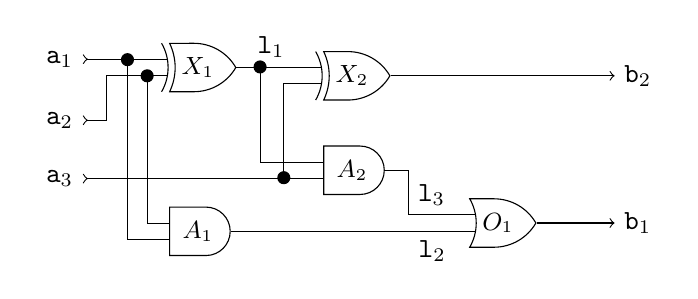
\begin{tikzpicture}[circuit logic US, minimum height=5mm]
\matrix[column sep=10mm]
{ \node[yshift=3pt] (i0) {$\texttt{a}_1$};& \node [xor gate] (xor1) {\small$X_1$};	& \node[yshift=-3pt,xor gate] (xor2) {\small$X_2$};	& 	& \node[yshift=-3pt] (o1) {$\texttt{b}_2$}; \\
\node[yshift=2pt] (i1) {$\texttt{a}_2$};&	& \node (cin) {};	&	&  \\
\node[yshift=-3pt] (i2) {$\texttt{a}_3$};&	& \node[and gate] (and1) {\small$A_2$};	&	& \\
	&	\node[and gate,yshift=-3pt] (and2) {\small$A_1$};	&	& \node[or gate] (or1) {\small$O_1$};	& \node (o2) {$\texttt{b}_1$};\\ };
\draw[>-] (i0.east) -- ++(right:3mm) |- (xor1.input 1);
\draw[*-] (xor1.input 1) ++(-5mm,0.8mm) |- (and2.input 2);
\draw[*-] (xor1.input 2) ++(-2.5mm,0.8mm) |- (and2.input 1) ;
\draw[>-] (i1.east) -- ++(right:3mm) |- (xor1.input 2);
\draw (xor1.output) -- ++(right:3mm) |- (xor2.input 1) node[midway,above,xshift=4pt,yshift=0pt] {$\texttt{l}_1$};
\draw[*-] (and1.input 1) ++(-5mm,-2.8mm) |- (xor2.input 2);
\draw[*-] (xor1.output) ++(3mm,0.9mm) |- (and1.input 1);
\draw[>-] (i2.east) -- ++(right:15mm) |- (and1.input 2);
\draw[->] (xor2.output) -- ++(right:3mm) |- (o1.west);
\draw (and1.output) -- ++(right:3mm) |- (or1.input 1) node[midway, above right ] {$\texttt{l}_3$};
\draw (and2.output) -- ++(right:3mm) |- (or1.input 2) node[near end,below right,xshift=+16pt] {$\texttt{l}_2$};
\draw[->] (or1.output) -- (o2.west);
\end{tikzpicture}
\caption{A two-bit full adder}
\label{fig:adder}
\end{figure}

The listing below shows a RankPL solution.
Line 1 encodes the space of possible inputs (0 or 1, equally likely).
The failure variables $\texttt{fa}_1$, $\texttt{fa}_2$, $\texttt{fo}_1$, $\texttt{fx}_2$ and $\texttt{fx}_2$ represent the events of individual gates failing and are set on line 2 (0 = OK, 1 = failing).
Here, we assume that failure is surprising to degree 1.
The circuit's logic is encoded on lines 3-7, where the output of a failing gate is arbitrarily set to 0 or 1.
Note that $\oplus$ stands for XOR.
At the end we observe $\phi$.

\noindent \begin{center}
\small
\begin{tabular}{rl}
\hline
1 & $\texttt{a}_1 := (0 \Rank{0} 1); \texttt{a}_2 := (0 \Rank{0} 1); \texttt{a}_3 := (0 \Rank{0} 1);$ \\
2 & $\texttt{fx}_1 := (0 \Rank{1} 1); \texttt{fx}_2 := (0 \Rank{1} 1); \texttt{fa}_1 := (0 \Rank{1} 1); \texttt{fa}_2 := (0 \Rank{1} 1); \texttt{fo}_1 := (0 \Rank{1} 1); $ \\
3 & $\textbf{if }\texttt{fx}_1 = 0\textbf{ then }\texttt{l}_1 := \texttt{a}_1 \oplus \texttt{a}_2\textbf{ else } \texttt{l}_1 := (0 \Rank{0} 1);$ \\
4 & $\textbf{if }\texttt{fa}_1 = 0\textbf{ then }\texttt{l}_2 := \texttt{a}_1 \wedge \texttt{a}_2\textbf{ else } \texttt{l}_2 := (0 \Rank{0} 1);$ \\
5 & $\textbf{if }\texttt{fa}_2 = 0\textbf{ then }\texttt{l}_3 := \texttt{l}_1 \wedge \texttt{a}_3\textbf{ else } \texttt{l}_3 := (0 \Rank{0} 1);$ \\
6 & $\textbf{if }\texttt{fx}_2 = 0\textbf{ then }\texttt{b}_2 := \texttt{l}_1 \oplus \texttt{a}_3\textbf{ else } \texttt{b}_2 := (0 \Rank{0} 1);$ \\
7 & $\textbf{if }\texttt{fo}_1 = 0\textbf{ then }\texttt{b}_1 := \texttt{l}_3 \vee \texttt{l}_2\textbf{ else } \texttt{b}_1 := (0 \Rank{0} 1);$ \\
8 & $\textbf{observe}\textbf{ }\phi;$\\
\hline
\end{tabular} \end{center} 

The different valuations of the failure variables produced by this program  
	represent explanations for the observation $\phi$, ranked according to plausibility.
Suppose we observe that the input $\texttt{a}_1\texttt{a}_2\texttt{a}_3$ is valued 001 while the output $\texttt{b}_1\texttt{b}_2$ is incorrectly valued 10 instead of 01.
Thus, we set $\phi$ to $\texttt{a}_1 = 0 \wedge \texttt{a}_2 = 0 \wedge \texttt{a}_3 = 1 \wedge \texttt{b}_1 = 1 \wedge \texttt{b}_2 = 0$.
This results in one outcome ranked 0, namely 
	$\texttt{fa}_1\texttt{fa}_2\texttt{fo}_1\texttt{fx}_2\texttt{fx}_2 = 00010$. % removed: inline
That is, $\phi$ is most plausibly explained by failure of $X_1$.
Other explanations are ranked higher than 0 and involve more than one faulty gate.\looseness=-1
% TODO: if space permits, elaborate on this example (belief revision, abduction)

%%%%%%%%%%%%%%%%%%%%%%%%%
%%%%%%%%%%%%%%%%%%%%%%%%%
\section{Noisy Observation and Iterated Revision}\label{sec:noisy}
%%%%%%%%%%%%%%%%%%%%%%%%%
%%%%%%%%%%%%%%%%%%%%%%%%%

%Plain conditioning works well if we accept that every piece of evidence $A$ is, after observation, 
%	believed with absolute certainty or, formally, that we have $\kappa_{A}(\overline{A}) = \infty$.
%However, if we have to deal with iterated belief change and noisy or possibly incorrect observations,
%	this becomes problematic.
%The reason is that revision by multiple contradicting observations is impossible:	
%	$(\kappa_{A})_{B}$ is undefined whenever $A \cap B = \emptyset$.
%In terms of RankPL, this means that the statement $\textbf{observe }a$ followed 
%	by the statement $\textbf{observe }b$ leads to failure whenever $a$ and $b$ are jointly unsatisfiable.
%To address this, a number of generalized forms of ranking-based conditioning have been proposed.
%In this section we discuss the two most prominent ones and we show how they can be expressed in RankPL,
%	using the \textbf{rank}, \textbf{observe} and default choice constructs as basic building blocks.
Conditioning by $A$ means that $A$ becomes believed with infinite firmness.
This is undesirable if we have to deal with iterated belief change or noisy or untrustworthy observations,
	since we cannot, after conditioning on $A$, condition on events inconsistent with $A$.
%There are a number of generalized forms of ranking-based conditioning that address this problem.
%In this section we discuss two of them, and show how they can be expressed in RankPL.
%%%%%%%%%%%%%%%%%%%%%%%%%
%\subsection{J-conditioning}
%%%%%%%%%%%%%%%%%%%%%%%%%
\emph{J-conditioning}~\cite{goldszmidt1996qualitative} is a more general form of conditioning that addresses this problem.
% (also called \emph{result-oriented} conditioning~\cite{DBLP:books/daglib/0035277}).
%It the ranking-based counterpart of the \emph{Jeffrey update rule} known from probability theory~\cite{goldszmidt1996qualitative}.
It is parametrized by a rank $x$ that indicates the firmness with which the evidence must be believed.
%It satisfies the DP postulates of iterated belief revision~\cite{DBLP:dblp_journals/ai/DarwicheP97}.\looseness=-1
%In the following definition we borrow notation from Spohn ~\cite{DBLP:books/daglib/0035277}.

\begin{definition}\label{defn:resultoriented}
Let $A \in \Omega$, $\kappa$ a ranking function over $\Omega$ such that $\kappa(A), \kappa(\overline A) < \infty$, and $x$ a rank.
The \emph{J-conditioning} of $\kappa$ by $A$ with strength $x$, denoted by $\kappa_{A \rightarrow x}$, is defined by
	$\kappa_{A \rightarrow x}(B) = min ( \kappa(B | A), \kappa(B | \overline A) + x ).$ % option: inline
\end{definition}

%This definition implies that $\kappa_{A \rightarrow x}(A) = 0$ and $\kappa_{A \rightarrow x}(\overline{A}) = x$.
%Thus, in words, the effect of J-conditioning by $A$ with strength $x$ is that $A$ becomes believed with firmness $x$. (TODO make sure firmness is defined)
%Note that J-conditioning generalizes plain conditioning, which is equivalent to J-conditioning with strength $\infty$.
%However, J-conditioning permits iterated belief change, 
%	because if the ranks of the possibilities contradicting the evidence are shifted up only by a finite number of ranks, 
%	the possibility that they get shifted down again afterwards is left open.
In words, the effect of J-conditioning by $A$ with strength $x$ is that $A$ becomes believed with firmness $x$.
This permits iterated belief change, because the rank of $\overline A$ is shifted up only by a finite number of ranks
	and hence can be shifted down again afterwards. %possibilities $A$ can still be shifted do.
%At this point we could introduce a special observe statement whose semantics corresponds to J-conditioning.
%We will not do that.
%Instead, we show that the basic language is already expressive enough
%	and that J-conditioning can be represented by combining 
%		two \textbf{observe} statements and a default choice construct.
%Let us state this formally.
%In what follows we write $\kappa_{b \rightarrow x}$ as shorthand for $\kappa_{\mods{\kappa}{b} \rightarrow x}$.
Instead of introducing a special statement representing J-conditioning, we show that we can already express it in RankPL.
Below we write $\kappa_{b \rightarrow x}$ as shorthand for $\kappa_{\mods{\kappa}{b} \rightarrow x}$.
Proofs are omitted due to space constraints.

\begin{theorem}
Let $b$ be a boolean expression and $\kappa$ a ranking function s.t. $\kappa(b) < \infty$ and $\kappa(\neg b) < \infty$.
We then have
$\kappa_{b \rightarrow x} = \dn{\textbf{observe }b \Rank{x} \textbf{observe }\neg b}(\kappa).$ % removed: inline
\end{theorem}

\emph{L-conditioning}~\cite{goldszmidt1996qualitative} %(also called \emph{evidence-oriented} conditioning~\cite{DBLP:books/daglib/0035277}) 
is another kind of generalized conditioning.
%It was first proposed by Shenoy~\cite{DBLP:journals/ijar/Shenoy91}.
%Again, it is a form of conditioning parametrized by a rank $x$.
Here, the parameter $x$ characterizes the `impact' of the evidence. %, rather than the firmness with which it must be believed.
%Again, we borrow notation from Spohn~\cite{DBLP:books/daglib/0035277}.\looseness=-1
%Again, it satisfies the DP postulates for iterated revision.\looseness=-1
\begin{definition}\label{defn:evidenceoriented}
Let $A \in \Omega$, $\kappa$ a ranking function over $\Omega$ such that $\kappa(A), \kappa(\overline A) < \infty$, and $x$ a rank.
The \emph{L-conditioning} of $\kappa$ is denoted by $\kappa_{A \uparrow x}$ and is defined by
	$\kappa_{A \uparrow x}(B) = min ( \kappa(A \cap B) - y, \kappa(\neg A \cap B) + x - y ),$ % removed: inline
where $y = min(\kappa(A), x).$
\end{definition}
Thus, L-conditioning by $A$ with strength $x$ means that $A$ improves by $x$ ranks w.r.t. the rank of $\neg A$.
%More precisely, the rank of $A$ is shifted down by $x$ units,
%	and if $A$ cannot be shifted down any further then $\neg A$ is shifted up by the remaining number of units.
%Like before, L-conditioning with strength $\infty$ is equivalent to plain conditioning.
Unlike J-conditioning, L-conditioning satisfies two properties 
that are desirable for modeling noisy observation:
	\textit{reversibility} ($(\kappa_{A \uparrow x})_{\overline{A} \uparrow x} = \kappa$) and 
	\textit{commutativity} ($(\kappa_{A \uparrow x})_{B \uparrow x} = (\kappa_{B \uparrow x})_{A \uparrow x}$)~\cite{DBLP:books/daglib/0035277}.
We now show how to express L-conditioning in RankPL.
Like before, we write $\kappa_{b \uparrow x}$ to denote $\kappa_{\mods{\kappa}{b} \uparrow x}$.
\begin{theorem}\label{thm:evidenceoriented}
Let $b$ be a boolean expression, $\kappa$ a ranking function over $\States$ such that $\kappa(b), \kappa(\neg b) < \infty$, and $x$ a rank.
We then have:
	$$\kappa_{b \uparrow x} = D
	\left\llbracket\begin{tabular}{c} 
	\mbox{$\textbf{if rank}(b) \leq x\textbf{ then}$} \\
	\mbox{$\textbf{observe }b \Rank{x - \textbf{rank}(b) + \textbf{rank}(\neg b)} \textbf{observe }\neg b$} \\
	\mbox{$\textbf{else}$} \\
	\mbox{$\textbf{observe }\neg b \Rank{\textbf{rank}(b) - x} \textbf{observe }b$} \\
	\end{tabular}\right\rrbracket(\kappa)$$
\end{theorem}
In what follows we use the statement $\textbf{observe}_{\textbf{L}}(b, x)$ as shorthand for the statement that represents L-conditioning as defined in theorem~\ref{thm:evidenceoriented}.
%\begin{proof}
%Let $A \in \Omega$, $\kappa$ a ranking function over $\Omega$ such that $\kappa(A), \kappa(\overline A) < \infty$, and $x$ be a rank.
%Two cases:
%\begin{itemize}
%\item $\kappa(b) \leq x$:
%	Definition~\ref{defn:evidenceoriented} then implies that $$\kappa_{b \uparrow x}(B) = min(\kappa_b(B), \kappa(\neg b \cap B) + x - \kappa(b)).$$
%	Because either $\kappa(b) = 0$ or $\kappa(\neg b) = 0$
%		we have that $x - \kappa(b) = - \kappa(\neg b) + (x - \kappa(b) + \kappa(\neg b))$.
%	From this it follows that 
%		$$\kappa_{b \uparrow x}(B) = min(\kappa_b(B), \kappa_{\neg b}(B) + (x - \kappa(b) + \kappa(\neg b)))$$
%	and hence
%		$$\kappa_{b \uparrow x}(B) = S[\textbf{observe }b \Rank{x - \textbf{rank}(b) + \textbf{rank}(\neg b)} \textbf{observe }\neg b](\kappa)(B).$$
%\item $x < \kappa(b)$:
%	Definition~\ref{defn:evidenceoriented} then implies that $$\kappa_{b \uparrow x}(B) = min ( \kappa(b \cap B) - x, \kappa(\neg b \cap B) ).$$
%	Furthermore we have $\kappa(\neg b) = 0$, and hence 
%		$$\kappa_{b \uparrow x}(B) = min ( \kappa_{\neg b}(B) , \kappa(b \cap B) - x).$$
%	From the fact $\kappa(b \cap B) = \kappa_{b}(B) + \kappa(b)$ it follows that
%		$$\kappa_{b \uparrow x}(B) = min ( \kappa_{\neg b}(B) , \kappa_{b}(B) + (\kappa(b) - x))$$
%	and hence 
%		$$\kappa_{b \uparrow x}(B) = S[\textbf{observe }\neg b \Rank{\textbf{rank}(b) - x} \textbf{observe }b](\kappa)(B).$$
%\end{itemize}
%\end{proof}

%%%%%%%%%%%%%%%%%%%%%%%%%
\subsubsection{Example}
%%%%%%%%%%%%%%%%%%%%%%%%%

The following problem involves both iterated revision and noisy observation.
A robot navigates a grid world and has to determine its location using a map and two distance sensors.
The grids in figure~\ref{fig:localization} depict the map that we use.
Gray cells represents walls and other cells are empty (ignoring, for now, the red cells and dots).
The sensors (oriented north and south) measure the distance to the nearest wall or obstacle.
To complicate matters, the sensor readings might not match the map.
For example, the $X$ in figure~\ref{fig:localization} marks an obstacle that affects sensor readings, but as far as the robot knows, this cell is empty.\looseness=-1

The listing below shows a RankPL solution.
The program takes as input:
(1) A map, held by an array\footnote{Semantically, arrays are just indexed variables.} $\texttt{map}$ of size $\texttt{n}\times \texttt{m}$, 
	storing the content of each cell (0 = empty, 1 = wall);
(2) An array $\texttt{mv}$ (length $\texttt{k}$) of movements (\texttt{N}/\texttt{E}/\texttt{S}/\texttt{W} for north/east/south/west) at given time points; and 
(3) Two arrays $\texttt{ns}$ and $\texttt{ss}$ (length $\texttt{k}$) with distances read by the north and south sensor at given time points.\looseness=-1

\noindent \begin{center}
\small
\begin{tabular}{rl}
\hline
1	& $\texttt{t} := 0; \texttt{ x} := 0 \Rank{0} \{1 \Rank{0} \{ 2 \Rank{0} \ldots \texttt{m}\} \}; \texttt{ y} := 0 \Rank{0} \{1 \Rank{0} \{ 2 \Rank{0} \ldots \texttt{n}\} \};$ \\
2	& $\textbf{while }(\texttt{t} \leq \texttt{k})\textbf{ do } \{$ \\
3	& \hspace{20pt}	$\textbf{if }(\texttt{mv}[\texttt{t}] = \texttt{N})\textbf{ then } \texttt{y} := \texttt{y} + 1$ \\
4	& \hspace{20pt}	$\textbf{else if }(\texttt{mv}[\texttt{t}] = \texttt{S})\textbf{ then } \texttt{y} := \texttt{y} - 1$ \\
5	& \hspace{20pt}	$\textbf{else if }(\texttt{mv}[\texttt{t}] = \texttt{W})\textbf{ then } \texttt{x} := \texttt{x} - 1$ \\
6	& \hspace{20pt}	$\textbf{else if }(\texttt{mv}[\texttt{t}] = \texttt{E})\textbf{ then } \texttt{x} := \texttt{x} + 1 \textbf{ else skip;}$ \\
7	& \hspace{20pt}	$\texttt{n} := 0; \textbf{ while }\texttt{map}[\texttt{x}][\texttt{y} + \texttt{n} + 1] = 0\textbf{ do }\texttt{n} := \texttt{n} + 1;$ \\
8	& \hspace{20pt}	$\textbf{observe}_{\textbf{L}}(1, \texttt{n} = \texttt{ns}[\texttt{t}]);$ \\
9	& \hspace{20pt}	$\texttt{s} := 0; \textbf{ while }\texttt{map}[\texttt{x}][\texttt{y} - \texttt{s} - 1] = 0\textbf{ do }\texttt{s} := \texttt{s} + 1;$ \\
10	& \hspace{20pt}	$\textbf{observe}_{\textbf{L}}(1, \texttt{s} = \texttt{ss}[\texttt{t}]);$ \\
11	& \hspace{20pt}	$\texttt{t} := \texttt{t} + 1;$\\
12	& $\}$ \\
\hline
\end{tabular} 
\end{center} 

The program works as follows.
On line 1 the robot's location $\texttt{x}$, $\texttt{y}$ is initialized to range over all coordinates
	using nested ranked choice statements.
The \textbf{while} loop iterates over the time point $\texttt{t}$ 
	and first processes the movement $\texttt{mv}[\texttt{t}]$ (lines 3-6).
On lines 7-8 the north sensor reading is processed
	by counting empty cells between the robot and nearest wall,
	the result of which is observed to equal $\texttt{ns}[\texttt{t}]$---and likewise for the south sensor (lines 9-10).
Here, we use L-conditioning with strength 1, to account for possible incorrect observations.
We then update $\texttt{t}$.\looseness=-1
\noindent \begin{figure}[t]
\centering
\begin{subfigure}[t]{0.24\columnwidth}
	\label{fig:localizationA}
	\centering
	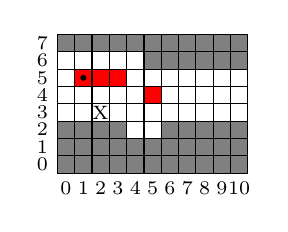
\begin{tikzpicture}[box/.style={rectangle,draw=black,thin, minimum size=1cm,scale=0.22},scale=0.22]	
	\foreach \x in {0,1,...,10}{
	    \foreach \y in {0,1,...,7}
	        \node[box] at (\x,\y){};
	}
	\foreach \i in {0,...,10} \node[below=3pt] at (\i,\yMin) {\scriptsize$\i$};
	\foreach \i in {0,...,7} \node[left=3pt] at (\xMin,\i) {\scriptsize$\i$};	
\node[box,fill=gray] at (0,0){};\node[box,fill=gray] at (1,0){};\node[box,fill=gray] at (2,0){};\node[box,fill=gray] at (3,0){};\node[box,fill=gray] at (4,0){};\node[box,fill=gray] at (5,0){};\node[box,fill=gray] at (6,0){};\node[box,fill=gray] at (7,0){};\node[box,fill=gray] at (8,0){};\node[box,fill=gray] at (9,0){};\node[box,fill=gray] at (10,0){};\node[box,fill=gray] at (0,1){};\node[box,fill=gray] at (1,1){};\node[box,fill=gray] at (2,1){};\node[box,fill=gray] at (3,1){};\node[box,fill=gray] at (4,1){};\node[box,fill=gray] at (5,1){};\node[box,fill=gray] at (6,1){};\node[box,fill=gray] at (7,1){};\node[box,fill=gray] at (8,1){};\node[box,fill=gray] at (9,1){};\node[box,fill=gray] at (10,1){};\node[box,fill=gray] at (0,2){};\node[box,fill=gray] at (1,2){};\node[box,fill=gray] at (2,2){};\node[box,fill=gray] at (3,2){};\node[box,fill=gray] at (6,2){};\node[box,fill=gray] at (7,2){};\node[box,fill=gray] at (8,2){};\node[box,fill=gray] at (9,2){};\node[box,fill=gray] at (10,2){};\node[box,fill=gray] at (5,6){};\node[box,fill=gray] at (6,6){};\node[box,fill=gray] at (7,6){};\node[box,fill=gray] at (8,6){};\node[box,fill=gray] at (9,6){};\node[box,fill=gray] at (10,6){};\node[box,fill=gray] at (0,7){};\node[box,fill=gray] at (1,7){};\node[box,fill=gray] at (2,7){};\node[box,fill=gray] at (3,7){};\node[box,fill=gray] at (4,7){};\node[box,fill=gray] at (5,7){};\node[box,fill=gray] at (6,7){};\node[box,fill=gray] at (7,7){};\node[box,fill=gray] at (8,7){};\node[box,fill=gray] at (9,7){};\node[box,fill=gray] at (10,7){};Iteration took 1 ms
	\node[font=\scriptsize] at (2,3) {X};
\node[box,fill=red] at (1,5){};\node[box,fill=red] at (5,4){};\node[box,fill=red] at (2,5){};\node[box,fill=red] at (3,5){};
	\fill (1,5) circle[radius=5pt] node {}; % \draw[->] (0,5) -- (1,5);
	\end{tikzpicture}
	\caption{$t = 1$}
\end{subfigure}
\begin{subfigure}[t]{0.24\columnwidth}
	\label{fig:localizationB}
	\centering
	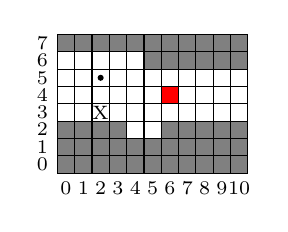
\begin{tikzpicture}[box/.style={rectangle,draw=black,thin, minimum size=1cm,scale=0.22},scale=0.22]	
	\foreach \x in {0,1,...,10}{
	    \foreach \y in {0,1,...,7}
	        \node[box] at (\x,\y){};
	}
	\foreach \i in {0,...,10} \node[below=3pt] at (\i,\yMin) {\scriptsize$\i$};
	\foreach \i in {0,...,7} \node[left=3pt] at (\xMin,\i) {\scriptsize$\i$};
\node[box,fill=gray] at (0,0){};\node[box,fill=gray] at (1,0){};\node[box,fill=gray] at (2,0){};\node[box,fill=gray] at (3,0){};\node[box,fill=gray] at (4,0){};\node[box,fill=gray] at (5,0){};\node[box,fill=gray] at (6,0){};\node[box,fill=gray] at (7,0){};\node[box,fill=gray] at (8,0){};\node[box,fill=gray] at (9,0){};\node[box,fill=gray] at (10,0){};\node[box,fill=gray] at (0,1){};\node[box,fill=gray] at (1,1){};\node[box,fill=gray] at (2,1){};\node[box,fill=gray] at (3,1){};\node[box,fill=gray] at (4,1){};\node[box,fill=gray] at (5,1){};\node[box,fill=gray] at (6,1){};\node[box,fill=gray] at (7,1){};\node[box,fill=gray] at (8,1){};\node[box,fill=gray] at (9,1){};\node[box,fill=gray] at (10,1){};\node[box,fill=gray] at (0,2){};\node[box,fill=gray] at (1,2){};\node[box,fill=gray] at (2,2){};\node[box,fill=gray] at (3,2){};\node[box,fill=gray] at (6,2){};\node[box,fill=gray] at (7,2){};\node[box,fill=gray] at (8,2){};\node[box,fill=gray] at (9,2){};\node[box,fill=gray] at (10,2){};\node[box,fill=gray] at (5,6){};\node[box,fill=gray] at (6,6){};\node[box,fill=gray] at (7,6){};\node[box,fill=gray] at (8,6){};\node[box,fill=gray] at (9,6){};\node[box,fill=gray] at (10,6){};\node[box,fill=gray] at (0,7){};\node[box,fill=gray] at (1,7){};\node[box,fill=gray] at (2,7){};\node[box,fill=gray] at (3,7){};\node[box,fill=gray] at (4,7){};\node[box,fill=gray] at (5,7){};\node[box,fill=gray] at (6,7){};\node[box,fill=gray] at (7,7){};\node[box,fill=gray] at (8,7){};\node[box,fill=gray] at (9,7){};\node[box,fill=gray] at (10,7){};Iteration took 1 ms
	\node[font=\scriptsize] at (2,3) {X};
\node[box,fill=red] at (6,4){};
	\fill (2,5) circle[radius=5pt] node {}; % \draw[->] (0,5) -- (2,5);
	\end{tikzpicture}
	\caption{$t = 2$}
\end{subfigure}
\begin{subfigure}[t]{0.24\columnwidth}
	\label{fig:localizationC}
	\centering
	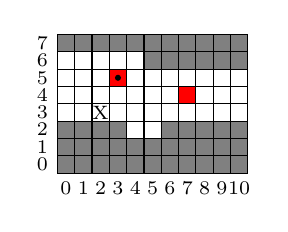
\begin{tikzpicture}[box/.style={rectangle,draw=black,thin, minimum size=1cm,scale=0.22},scale=0.22]	
	\foreach \x in {0,1,...,10}{
	    \foreach \y in {0,1,...,7}
	        \node[box] at (\x,\y){};
	}
	\foreach \i in {0,...,10} \node[below=3pt] at (\i,\yMin) {\scriptsize$\i$};
	\foreach \i in {0,...,7} \node[left=3pt] at (\xMin,\i) {\scriptsize$\i$};
\node[box,fill=gray] at (0,0){};\node[box,fill=gray] at (1,0){};\node[box,fill=gray] at (2,0){};\node[box,fill=gray] at (3,0){};\node[box,fill=gray] at (4,0){};\node[box,fill=gray] at (5,0){};\node[box,fill=gray] at (6,0){};\node[box,fill=gray] at (7,0){};\node[box,fill=gray] at (8,0){};\node[box,fill=gray] at (9,0){};\node[box,fill=gray] at (10,0){};\node[box,fill=gray] at (0,1){};\node[box,fill=gray] at (1,1){};\node[box,fill=gray] at (2,1){};\node[box,fill=gray] at (3,1){};\node[box,fill=gray] at (4,1){};\node[box,fill=gray] at (5,1){};\node[box,fill=gray] at (6,1){};\node[box,fill=gray] at (7,1){};\node[box,fill=gray] at (8,1){};\node[box,fill=gray] at (9,1){};\node[box,fill=gray] at (10,1){};\node[box,fill=gray] at (0,2){};\node[box,fill=gray] at (1,2){};\node[box,fill=gray] at (2,2){};\node[box,fill=gray] at (3,2){};\node[box,fill=gray] at (6,2){};\node[box,fill=gray] at (7,2){};\node[box,fill=gray] at (8,2){};\node[box,fill=gray] at (9,2){};\node[box,fill=gray] at (10,2){};\node[box,fill=gray] at (5,6){};\node[box,fill=gray] at (6,6){};\node[box,fill=gray] at (7,6){};\node[box,fill=gray] at (8,6){};\node[box,fill=gray] at (9,6){};\node[box,fill=gray] at (10,6){};\node[box,fill=gray] at (0,7){};\node[box,fill=gray] at (1,7){};\node[box,fill=gray] at (2,7){};\node[box,fill=gray] at (3,7){};\node[box,fill=gray] at (4,7){};\node[box,fill=gray] at (5,7){};\node[box,fill=gray] at (6,7){};\node[box,fill=gray] at (7,7){};\node[box,fill=gray] at (8,7){};\node[box,fill=gray] at (9,7){};\node[box,fill=gray] at (10,7){};Iteration took 1 ms
	\node[font=\scriptsize] at (2,3) {X};
\node[box,fill=red] at (3,5){};\node[box,fill=red] at (7,4){};
	\fill (3,5) circle[radius=5pt] node {}; % \draw[->] (0,5) -- (3,5);
	\end{tikzpicture}
	\caption{$t = 3$}
\end{subfigure}
\begin{subfigure}[t]{0.24\columnwidth}
	\label{fig:localizationD}
	\centering
	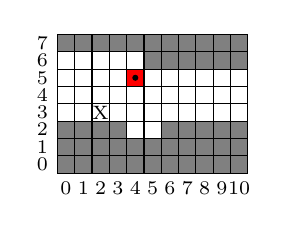
\begin{tikzpicture}[box/.style={rectangle,draw=black,thin, minimum size=1cm,scale=0.22},scale=0.22]	
	\foreach \x in {0,1,...,10}{
	    \foreach \y in {0,1,...,7}
	        \node[box] at (\x,\y){};
	}
	\foreach \i in {0,...,10} \node[below=3pt] at (\i,\yMin) {\scriptsize$\i$};
	\foreach \i in {0,...,7} \node[left=3pt] at (\xMin,\i) {\scriptsize$\i$};
\node[box,fill=gray] at (0,0){};\node[box,fill=gray] at (1,0){};\node[box,fill=gray] at (2,0){};\node[box,fill=gray] at (3,0){};\node[box,fill=gray] at (4,0){};\node[box,fill=gray] at (5,0){};\node[box,fill=gray] at (6,0){};\node[box,fill=gray] at (7,0){};\node[box,fill=gray] at (8,0){};\node[box,fill=gray] at (9,0){};\node[box,fill=gray] at (10,0){};\node[box,fill=gray] at (0,1){};\node[box,fill=gray] at (1,1){};\node[box,fill=gray] at (2,1){};\node[box,fill=gray] at (3,1){};\node[box,fill=gray] at (4,1){};\node[box,fill=gray] at (5,1){};\node[box,fill=gray] at (6,1){};\node[box,fill=gray] at (7,1){};\node[box,fill=gray] at (8,1){};\node[box,fill=gray] at (9,1){};\node[box,fill=gray] at (10,1){};\node[box,fill=gray] at (0,2){};\node[box,fill=gray] at (1,2){};\node[box,fill=gray] at (2,2){};\node[box,fill=gray] at (3,2){};\node[box,fill=gray] at (6,2){};\node[box,fill=gray] at (7,2){};\node[box,fill=gray] at (8,2){};\node[box,fill=gray] at (9,2){};\node[box,fill=gray] at (10,2){};\node[box,fill=gray] at (5,6){};\node[box,fill=gray] at (6,6){};\node[box,fill=gray] at (7,6){};\node[box,fill=gray] at (8,6){};\node[box,fill=gray] at (9,6){};\node[box,fill=gray] at (10,6){};\node[box,fill=gray] at (0,7){};\node[box,fill=gray] at (1,7){};\node[box,fill=gray] at (2,7){};\node[box,fill=gray] at (3,7){};\node[box,fill=gray] at (4,7){};\node[box,fill=gray] at (5,7){};\node[box,fill=gray] at (6,7){};\node[box,fill=gray] at (7,7){};\node[box,fill=gray] at (8,7){};\node[box,fill=gray] at (9,7){};\node[box,fill=gray] at (10,7){};Iteration took 1 ms
	\node[font=\scriptsize] at (2,3) {X};
\node[box,fill=red] at (4,5){};
	\fill (4,5) circle[radius=5pt] node {}; % \draw[->] (0,5) -- (4,5);
	\end{tikzpicture}
	\caption{$t = 4$}
\end{subfigure}
\caption{Most plausible inferred locations during four iterations}
\label{fig:localization}
\end{figure}

The different values for $\texttt{x},\texttt{y}$ generated by this program encode possible locations of the robot, ranked according plausibility.
Suppose the robot moves from $(0,5)$ to $(4, 5)$.
Thus, we set $\texttt{mv} = \{ E, E, E, E \}$, $\texttt{ns} = \{ 1, 1, 1, 1 \}$ and $\texttt{ss} = \{ 2, 1, 2, 3 \}$.
The dots in figure~\ref{fig:localization} show robot's position after each step,
	while the red cells represent the inferred most plausible (i.e., rank zero) locations.
If we terminate at $t = 1$ (i.e., we set $k$ to $0$) we get four locations,
	all of which are consistent with the observed distances 1 (north) and 2 (south).
After two iterations, the robot wrongly believes to be at (6, 4), due to having observed the obstacle.
However, after two more iterations, the robot found its actual location.\looseness=-1

Note that using L-conditioning here is essential.
Regular conditioning would cause failure after the third iteration. 
We could also have used J-conditioning, which gives different rankings of intermediate results.

\section{Implementation}\label{sec:implementation}

A RankPL interpreter written in Java can be found at \url{http://github.com/tjitze/RankPL}.
It runs programs written using the syntax described in this paper, 
	or constructed using Java classes that map to this syntax.
The latter makes it possible to embed RankPL programs inside Java code
	and to make it interact with and use classes and methods written Java.
The interpreter is faithful to the semantics described in section~\ref{sec:rpl} and
	implements the \emph{most-plausible-first} execution strategy discussed in section~\ref{sec:formalsemantics}.
All examples discussed in this paper are included, as well as a number of additional examples.

\section{Conclusion and Future Work}\label{sec:conclusion}

We have introduced RankPL, a language semantically similar to probabilistic programming,
	but based on Spohn's ranking theory,
	and demonstrated its utility using examples involving abduction and iterated revision.
We believe that the approach has great potential for applications
	where PPLs are too demanding due to their computational complexity and dependence on precise probability values.
Moreover, we hope that our approach will generate a broader and more practical scope for the topics of 
	ranking theory and belief revision which, in the past, have been studied mostly from purely theoretical perspectives.

A number of aspects were not touched upon and will be addressed in future work.
This includes a more fine grained characterization of termination
	and a discussion of the relationship with nondeterministic programming, 
	which is a special case of RankPL.
Furthermore, we have omitted examples to show that RankPL
	subsumes ranking networks 
	and can be used to reason about causal rules and actions~\cite{goldszmidt1996qualitative}.
We also did not contrast our approach 
	with default reasoning formalisms that use ranking theory as a semantic foundation (see, e.g.,~\cite{DBLP:conf/tark/Pearl90}).

Even though we demonstrated that RankPL is expressive enough to solve 
	fairly complex tasks in a compact manner, it is a very basic language that is best regarded as proof of concept.
In principle, the approach can be applied to any programming language,
	whether object-oriented, functional, or LISP-like.
Doing so would make it possible to reason about ranking-based models expressed using, for example, recursion and complex data structures.
These features are also supported by PPLs such as Church~\cite{DBLP:conf/uai/GoodmanMRBT08}, 
	Venture~\cite{DBLP:journals/corr/MansinghkaSP14} and Figaro~\cite{pfeffer2009figaro}. 
	


%% The Appendices part is started with the command \appendix;
%% appendix sections are then done as normal sections
%% \appendix

%% \section{}
%% \label{}

%% If you have bibdatabase file and want bibtex to generate the
%% bibitems, please use
%%
%%  \bibliographystyle{elsarticle-num} 
%%  \bibliography{<your bibdatabase>}

%% else use the following coding to input the bibitems directly in the
%% TeX file.

\bibliography{bibliography}

\end{document}